\section{Results}
\label{sec:results}

In this section, we numerically evaluate the quantum resources required for block-encoding various operators using LOBE.
The spacetime costs that we analyze include: the number of T gates, the number of non-Clifford single qubit rotations, the number of block-encoding ancillae, the maximum number of qubits required, and the rescaling factor imposed on the resulting block-encoding.

We compare the LOBE constructions presented in Section \ref{sec:ladder-op-oracles} to techniques that first expand the ladder operators in the Pauli basis and then block-encode the resulting linear combinations of Pauli operators using LCU.
The Jordan-Wigner transformation \cite{jordan-wigner} is used to expand fermionic ladder operators in the basis of Pauli operators, while, the Standard Binary encoding \cite{standard-binary} is used to expand bosonic ladder operators.

The first LCU-based method we compare against will be referred to as ``LCU - Expansion''.
In this method, the respective Pauli transformations are applied to the ladder operators and fully expanded, resulting in a single linear combination of Pauli operators.
This linear combination, which describes the full operator, is then block-encoded using the LCU framework.

The second LCU-based method we compare against will be referred to as ``LCU - Piecewise''.
In this method, each individual ladder operator is expanded in the Pauli basis and then block-encoded using the LCU framework.
These block-encodings of individual ladder operators are then combined together to produce a block-encoding of the full operator using the techniques described in subsections \ref{subsec:lco} and \ref{subsec:be-products}.

In the following subsections, we benchmark these three different block-encoding methods for various types of operators.
First, we analyze the associated spacetime costs for block-encoding several classes of operators which appear in many second-quantized operators.
Then, we present the spacetime costs for block-encoding Hamiltonians associated with various models that arise in quantum field theory.
These models include Hamiltonians derived from two non-relativistic models - the quartic harmonic oscillator and the static massive Yukawa - and two fully relativistic models - $\phi^4$ theory and the full massive Yukawa.

The results that we present in this section are generated by constructing the circuits using Cirq \cite{cirq} and constructions are numerically verified for circuits up to 18 qubits.
The operators are constructed through the use of OpenParticle \cite{openparticle}, a software library for the construction and manipulation of fermionic, antifermionic, and bosonic ladder operators.
The Symmer software library \cite{} is also used for various subroutines, including, but not limited to, expanding the ladder operators in the Pauli basis.
The software library \cite{grover-rudolph-github} is used to determine the rotation angles required for Grover-Rudolph.

\subsection{Components}

In this subsection, we numerically benchmark the spacetime cost of LOBE constructions in comparison with the two LCU methods outlined above for three different sets of operators.

\begin{figure*}
    \centering
    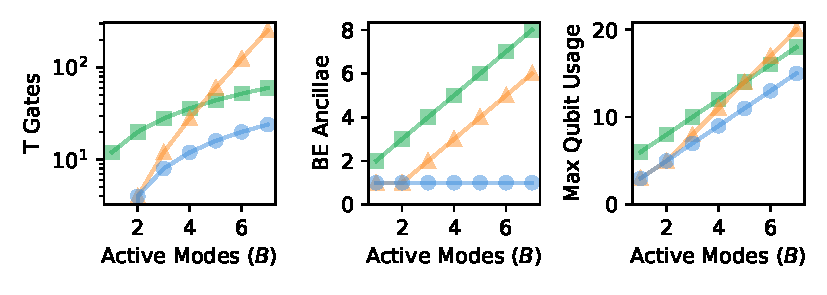
\includegraphics[width=12cm]{figures/fermionic-hc-comparison.pdf}
    \caption{
        \textbf{Spacetime Cost to Block-Encode $O = b_0 b_1 \hdots b_{B-1} + h.c.$}
        The number of T gates (left), block-encoding ancillae (middle), and maximum number of qubits used (right) are shown as a function of the number of active modes ($B$).
        Results for ``LCU - Expansion'' are shown as the orange triangles, results for ``LCU - Piecewise'' are shown as the green squares, and results for LOBE are shown as the blue circles.
        For this operator, all block-encodings use zero non-Clifford rotations.
        Both ``LCU - Expansion'' and LOBE have optimal rescaling factors ($\lambda = 1$) while ``LCU - Piecewise'' has a rescaling factor of $\lambda = 2$.
    }
    \label{fig:fermionic-hc-comparison}
\end{figure*}

The first set of operators we examine are described by a product of fermionic annihilation operators acting on different modes plus its hermitian conjugate: $b_0 b_1 \hdots b_{B-1} + h.c.$.
The numerical spacetime costs of the three block-encoding methods for these operators are shown as a function of the number of active modes ($B$) in Figure \ref{fig:fermionic-hc-comparison}.
Notably, the spacetime costs for LOBE and ``LCU - Expansion'' are identical for $B = 1$ and $B = 2$.
However, the number of required T gates scales exponentially with $B$ for ``LCU - Expansion'', yet scales linearly for LOBE.
Additionally, the LOBE constructions only require a single block-encoding ancilla regardless of $B$ while both LCU methods require a number of block-encoding ancillae that scale linearly with $B$.

\begin{figure*}
    \centering
    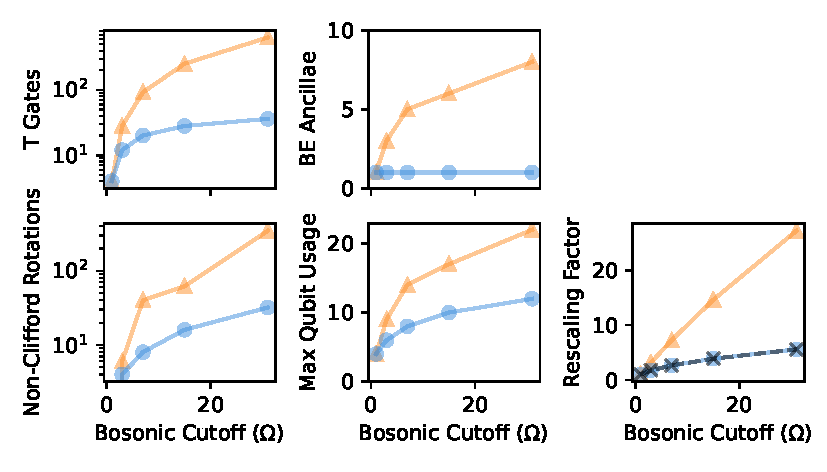
\includegraphics[width=14cm]{figures/bosonic-comparison.pdf}
    \caption{
        \textbf{Spacetime Cost to Block-Encode Bosonic Annihilation Operator}
        The number of T gates (upper-left), number of non-Clifford rotations (lower-left), block-encoding ancillae (upper-middle), maximum number of qubits used (lower-middle), and rescaling factor (lower-right) are shown as a function of the bosonic occupation cutoff ($\Omega$).
        Results for LCU are shown as the orange triangles and results for LOBE are shown as the blue circles.
        The optimal rescaling factor, which is given by the L2 norm of the matrix representing the bosonic annihilation operator with fixed $\Omega$, is shown as the dashed black crosses. 
    }
    \label{fig:bosonic-comparison}
\end{figure*}

The second set of block-encodings we consider is those that encode a single bosonic annihilation operator ($a$) with an increasing bosonic occupation cutoff ($\Omega$).
Since there is only a single operator, both LCU methods result in the same construction therefore we refer to these constructions by ``LCU''.
The numerical spacetime costs and rescaling factors of the LCU and LOBE block-encodings are shown in Figure \ref{fig:bosonic-comparison}.
The LOBE constructions result in block-encodings with fewer required resources for all metrics as compared to LCU.
Notably, the number of required T gates scales logarithmically with $\Omega$ for LOBE, yet scales roughly linearly for LCU.
Additionally, the number of block-encoding ancillae is constant ($1$) regardless of $\Omega$ for LOBE, yet scales logarithmically for LCU.
Lastly, the LOBE construction results in a rescaling factor that matches the operator norm (optimal), while the LCU construction results in a larger rescaling factor.

\begin{figure*}
    \centering
    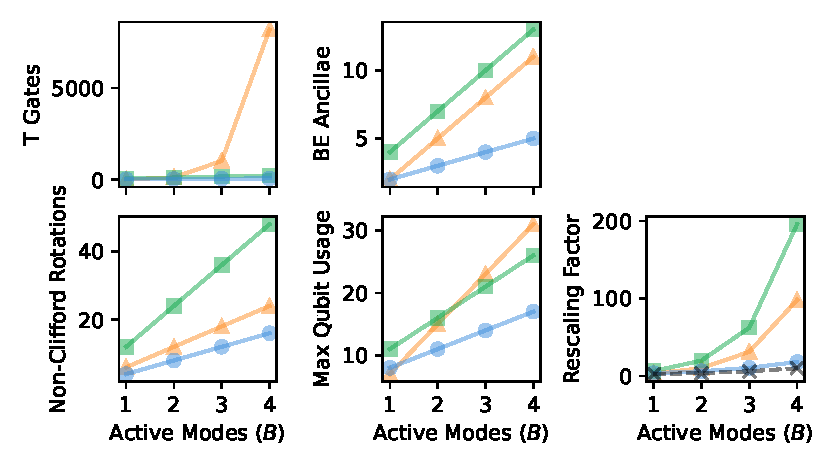
\includegraphics[width=14cm]{figures/bosonic-hc-comparison.pdf}
    \caption{
        \textbf{Spacetime Cost to Block-Encode $O = a_0 a_1 \hdots a_{B-1} + h.c.$}
        The number of T gates (upper-left), number of non-Clifford rotations (lower-left), block-encoding ancillae (upper-middle), maximum number of qubits used (lower-middle), and rescaling factor (lower-right) are shown as a function of the number of active modes ($B$).
        The bosonic cutoff is fixed to $\Omega = 3$ for all data points.
        Results for ``LCU - Expansion'' are shown as the orange triangles, results for ``LCU - Piecewise'' are shown as the green squares, and results for LOBE are shown as the blue circles.
        The optimal rescaling factor, which is given by the L2 norm of the matrix representing the operator with $\Omega = 3$, is shown as the dashed black crosses.
    }
    \label{fig:bosonic-hc-comparison}
\end{figure*}

The third set of operators we analyze are given as a linear combination of a product of bosonic annihilation operators acting on different modes plus its hermitian conjugate: $a_0 a_1 \hdots a_{B-1} + h.c.$.
The numerical spacetime costs of the various block-encoding constructions for these operators with $\Omega = 3$ are shown in Figure \ref{fig:bosonic-hc-comparison}.
Notably, the overall time-complexity scales linearly with $B$ for the LOBE and ``LCU - Piecewise'' constructions, while it scales exponentially for ``LCU - Expansion''.
For the space complexity metrics, all methods scale linearly with $B$, yet the LOBE constructions have both the smallest prefactor and numerical values.
Finally, the LOBE construction results in the lowest rescaling factor of all constructions.

\subsection{Quartic Harmonic Oscillator Results}
\label{sec:qosc_results}

The quartic harmonic oscillator \cite{PhysRev.184.1231, girguś2024spiralflowquantumquartic, wójcik2012applicationnumericalrenormalizationgroup} is an extension of the standard harmonic oscillator with an additional non-linearity of the form $g \varphi^4$, where $g$ is an arbitrary constant that dictates the strength of the interaction, and $\phi$ is a bosonic field.
This leads to the Hamiltonian $H = \frac12\dot\phi^2 + \frac{m}{2}\phi^2 + gm^3\phi^4 $, where $\phi$ is composed of a single mode.
$m$ is the mass of the bosonic particle, and $\dot \phi$ represents the time derivate of the field.

In a second-quantized, dimensionless form, the Hamiltonian can be written as:
\begin{equation}
    \label{eq:qosc}
    H = a^\dagger a + g\left(a + a^\dagger \right)^4
\end{equation}
where there is only one bosonic mode.

After expanding the product, normal ordering all terms, and removing the constant offset, this Hamiltonian can be written as a linear combination of $8$ terms consisting of three pairs of operators plus their hermitian conjugates and two operators that are their own hermitian conjugates:
\begin{equation}
    \begin{split}
        H = &(12g + 1) a^\dagger a + 6g a^{\dagger^2} a^2 + 6g \left(a^{\dagger^2} + a^2 \right) \\
        + &4g \left(a^{\dagger^3} a + a^\dagger a^3 \right) + g \left(a^{\dagger^4} + a^4 \right)
    \end{split}
\end{equation}

\begin{figure*}
    \label{fig:qosc}
    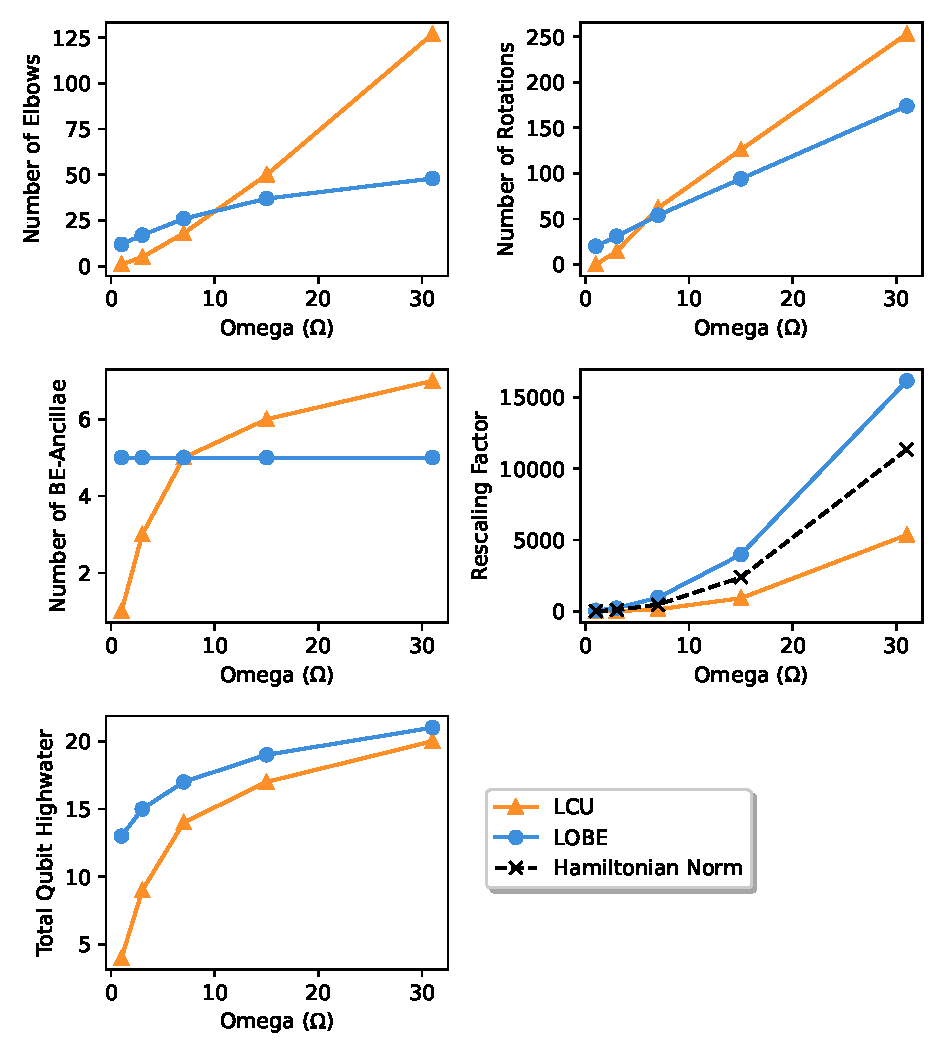
\includegraphics[width = 16cm]{figures/quartic_oscillator.pdf}
    \caption{
        \textbf{Quartic Harmonic Oscillator}
        The number of T gates (upper-left), number of non-Clifford rotations (lower-left), block-encoding ancillae (upper-middle), maximum number of qubits used (lower-middle), and rescaling factor (lower-right) are shown as a function of the bosonic occupation cutoff ($\Omega$).
        The parameter $g$ is set to $1$ for all data points.
        Results for the Pauli Expansion method are shown as the orange triangles and results for LOBE are shown as the blue circles.
        The optimal rescaling factor, which is given by the L2 norm of the Hamiltonian, is shown as the dashed black crosses.
    }
\end{figure*}

In Figure \ref{fig:qosc}, we show the scaling of the spacetime costs associated with both the LOBE and Pauli Expansion block-encodings as a function of the bosonic occupation cutoff ($\Omega$).
For small values of $\Omega$, the Pauli Expansion block-encodings result in lower spacetime costs, however, the LOBE constructions have favorable scaling and therefore a crossover point is seen.

For the time-complexity, this crossover occurs at $\Omega = 15$ for the number of T gates and $\Omega = 7$ for the number of non-Clifford rotations.
For the space-complexity, this crossover occurs at $\Omega = 7$ for the number of block-encoding ancillae and $\Omega = 31$ for the maximum number of qubits.
Finally, for the rescaling factor, this crossover occurs at $\Omega = 31$.

\subsection{Massive Static Yukawa}
\label{sec:static_yukawa}

The next simplest model that we consider is a non-relativistic approximation to the Yukawa model, which is commonly referred to as the massive static Yukawa model \cite{PhysRevD.103.014021}.
This model is taken as the limit of the full Yukawa model of infinitely heavy fermions, and bosons at rest relative to the fermions that emit/absorb them.

The second-quantized Hamiltonian for this model is given by:
\begin{equation}
    \label{eq:static-yukawa}
    H = C_f b^\dagger b + C_b a^\dagger a + g b^\dagger b \left( a + a^\dagger \right)
\end{equation}
where $C_f$ ..., $C_b$ ..., and $g$ ... \ws{@Gus}.
In this model, there is one fermionic mode and one bosonic mode so the indices on each mode are omitted. 

\begin{figure*}
    \label{fig:static_yukawa}
    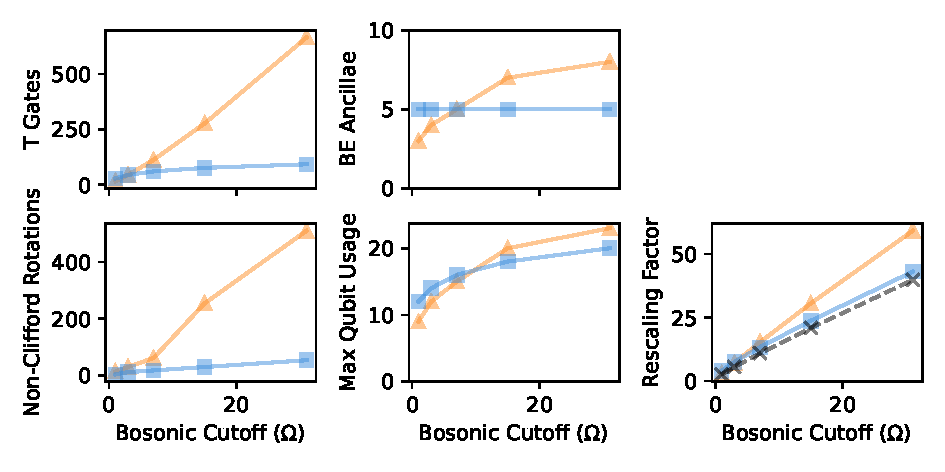
\includegraphics[width = 16cm]{figures/static_yukawa.pdf}
    \caption{
        \textbf{Static Massive Yukawa}
        The number of T gates (upper-left), number of non-Clifford rotations (lower-left), block-encoding ancillae (upper-middle), maximum number of qubits used (lower-middle), and rescaling factor (lower-right) are shown as a function of the bosonic occupation cutoff ($\Omega$).
        The parameters $C_f$, $C_b$, and $g$ are set to $1$ for all data points.
        Results for the Pauli Expansion method are shown as the orange triangles and results for LOBE are shown as the blue circles.
        The L2 norm of the Hamiltonian is shown as the dashed black crosses.
    }
\end{figure*}

As this model is restricted to one fermionic and one bosonic mode, we compare the spacetime costs of the different block-encoding methods as a function of the bosonic occupation cutoff ($\Omega$).
Similar to the quartic harmonic oscillator, the Pauli Expansion method results in lower spacetime costs when the bosonic cutoff is low.
However, the LOBE constructions have better asymptotic scaling with resect to $\Omega$ and crossover points exist for all metrics, above which LOBE results in lower cost constructions.

For the time-complexity, this crossover point occurs at $\Omega = 3$ for the number of T gates and the LOBE constructions require fewer non-Clifford rotations at all values of $\Omega$.
For the space-complexity, this crossover point occurs at $\Omega = 7$ for the number of block-encoding ancillae and $\Omega = 15$ for the maximum number of qubits.
Finally, for the rescaling factor, this crossover point occurs at $\Omega = 15$.
\subsection{$\phi^4$ Results}
\label{sec:phi4_results}

Any field theory is defined at the level of a Lagrangian.
For $\phi^4$ theory is given as
\begin{equation}
    \mathcal{L} = \frac12 \left(\partial_\mu \phi \right)^2 - \frac{m^2}{2}\phi^2 - g\phi^4.
\end{equation}

To obtain a Hamiltonian from a Lagrangian, a Legendre transformation is performed, in which an explicit set of coordinates must be chosen. 
The set of coordinates used in this paper, which lead to the simplest forms of the corresponding Hamiltonians, are front form (lightfront) coordinates \cite{Dirac1949}.
A discussion on lightfront coordinates will be given in appendix \ref{subsec:qft-hamiltonians}.

The $\phi^4$ Hamiltonian can be written as:
\begin{align}
    H = \sum_i &c_i a_i^\dagger a_i + \sum_{ijkl}c_{ijkl} \left(a_i^\dagger a_j^\dagger a_k^\dagger a_l + h.c. \right) + \nonumber\\
    &\sum_{ijkl}c_{ijkl}a_i^\dagger a_j^\dagger a_k a_l
\end{align}
where the values of the coefficients are omitted for brevity, but can be determined numerically.

Unlike the Quartic Harmonic Oscillator and the Static Massive Yukawa model, $\phi^4$ theory is defined based on a discretization of momentum modes.
In lightfront field theories, it is common to refer to the resolution of the model, which dictates the size of the momentum grid or the total number of momentum modes.
For those unfamiliar, the resolution can be thought of analogously to the molecular orbital basis in quantum chemistry simulations.
A further discussion on the physical meaning of resolution will be given in appendix \ref{subsec:qft-hamiltonians}.

\begin{figure*}
    \label{fig:phi4}
    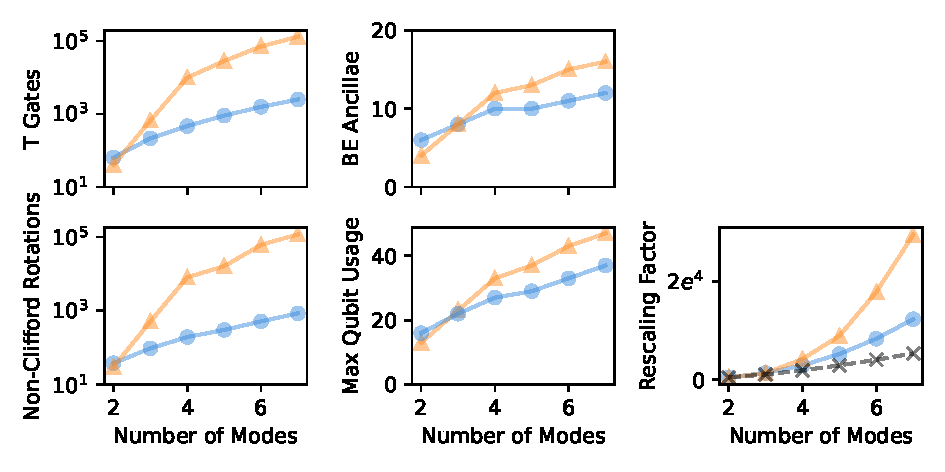
\includegraphics[width = 16cm]{figures/phi4-resolution-3.pdf}
    \caption{
        \textbf{$\phi^4$}
        The number of T gates (upper-left), number of non-Clifford rotations (lower-left), block-encoding ancillae (upper-middle), maximum number of qubits used (lower-middle), and rescaling factor (lower-right) are shown as a function of the number of momentum modes.
        The bosonic cutoff is fixed to $\Omega = 3$ and the parameters $g$ and $m_b$ are set to $1$ for all data points.
        Results for the ``Pauli - Expansion" method are shown as the orange triangles and results for LOBE are shown as the blue circles.
        The optimal rescaling factor, which is given by the L2 norm of the Hamiltonian, is shown as the dashed black crosses.
    }
\end{figure*}

Since the previous results establish that LOBE constructions are generally preferred when the bosonic cutoff is large, here we chose to look at the spacetime cost as a function of the total number of momentum modes.
In Figure \ref{fig:phi4}, we show the scaling of the spacetime costs associated with both the LOBE and Pauli Expansion block-encodings as a function of the number of modes.
For these estimates, the bosonic cutoff is fixed to $\Omega = 3$.
When the number of modes is small (low resolution), the LOBE and Pauli Expansion constructions require similar spacetime costs, with the Pauli Expansion block-encodings requiring \ws{one} fewer block-encoding ancilla when there are only two modes.
For higher resolutions (more modes), the LOBE constructions require signficantly fewer T gates and non-Clifford rotations, in addition to requiring fewer block-encoding ancillae, using fewer total qubits, and having smaller rescaling factors.
Notably, when $7$ momentum modes are used, the time cost for the LOBE construction is approximately two orders of magnitude smaller than the Pauli Expansion construction.

\subsection{Full Yukawa Results}
\label{sec:yukawa_results}

The first interacting field theory between different types of particles studied is generally the Yukawa model.
This is a theory of interacting fermions and bosons which can be used as a model of the strong nuclear force between hadrons.
The Lagrangian for this model is given as

\begin{equation}
    \label{eq:yukawa-lagrangian}
    \mathcal{L} = \bar \psi \left(i\gamma^\mu \partial_\mu - m \right)\psi + \frac{1}{2}\partial_\mu \phi \partial^\mu \phi - \frac{1}{2}\mu^2\phi^2 - g\bar \psi \psi \phi,
\end{equation}

The Hamiltonian can be written, again with coefficients obscured, as:

\begin{align}
    \begin{split}
        H = &\sum_i c_i b_i^\dagger b_i + \sum_i c_i d_i^\dagger d_i + \sum_i c_i a_i^\dagger a_i + \\
        &\sum_{ijk}c_{ijk}\left(b_i^\dagger b_j a_k^\dagger + h.c. \right) + \sum_{ijk}c_{ijk}\left(d_i^\dagger d_j a_k^\dagger + h.c. \right) + \\
        &\sum_{ijk}c_{ijk}\left(b_i^\dagger d_j^\dagger a_k + h.c. \right) + \sum_{ijkl}c_{ijkl}b_i^\dagger b_j a_k^\dagger a_l + \\
        &\sum_{ijkl}c_{ijkl}d_i^\dagger d_j a_k^\dagger a_l + \sum_{ijkl}c_{ijkl}\left(b_i^\dagger d_j^\dagger a_k a_l + h.c. \right)
    \end{split}
\end{align}

Unlike $\phi^4$ theory, the Yukawa model involves another type of field, a fermionic (Dirac) field $\psi$ describing fermionic particles.
$\bar \psi$ is the conjugate Dirac field, $m_f$ is the mass of the fermion, $m_b$ is the mass of the boson, and $g$ again describes the strength of the interaction.

% \subsection{Yukawa Theory}
% A quantum field theory that models the strong nuclear force between hadrons is Yukawa theory \cite{Peskin:1995ev}. In this theory, hadrons are described by a fermionic field $\psi$, coupled via a scalar boson $\phi$. The interaction term is $\mathcal{L}_{\text{Yukawa}} = g\bar\psi \psi \phi$, which leads to interaction vertices containing fermions and/or antifermions and bosons. The Lagrangian, and thus the Hamiltonian, is written as a sum of free, non-ineteracting fields and the interaction term.
% The first two models below can be thought of as corresponding to a full quantum field theory constrained to a single mode, reducing it to a quantum mechanics problem.

% In this section, we demonstrate the use of LOBE to block-encode Hamiltonians derived from quantum field theories: Yukawa theory and $\phi^4$ theory \cite{Peskin:1995ev}.
% We study both variants of the block-encoding described in Sections \ref{sec:block-encoding} and expanded upon in Section \ref{sec:lobe} and give numerical counts for the numbers of non-Clifford operations, the number of ancillae required beyond the system register, and the rescaling factor imposed on the resulting block-encoding.

% The results that we present here are generated based on constructions of LOBE that are written in Cirq \cite{cirq} and the block-encodings are numerically verified for circuits of up to 14 qubits.
% Additionally, the operators are constructed through the use of OpenParticle \cite{openparticle}, a software library for the construction and manipulation of fermionic, antifermionic, and bosonic ladder operators.
% The software library \cite{grover-rudolph-github} is used to determine the rotation angles required for Grover-Rudolph.

% \subsection{Yukawa Theory}
% A quantum field theory that models the strong nuclear force between hadrons is Yukawa theory \cite{Peskin:1995ev}. In this theory, hadrons are described by a fermionic field $\psi$, coupled via a scalar boson $\phi$. The interaction term is $\mathcal{L}_{\text{Yukawa}} = g\bar\psi \psi \phi$, which leads to interaction vertices containing fermions and/or antifermions and bosons. The Lagrangian, and thus the Hamiltonian, is written as a sum of free, non-ineteracting fields and the interaction term.

% Utilizing the lightfront frame \cite{Dirac1949}, leads to a straightforward approach to writing down the Hamiltonian bound-state eigenvalue equation in terms of ladder operators. This lightfront frame removes the ambiguous $\sqrt{\nabla^2 + m^2}$ term that appears in a canonical, instant-time frame Hamiltonian approach. 

% The interaction terms in the Hamiltonian are $H_{\text{Yukawa int}} \in \{b^\dagger b a, b^\dagger b a^\dagger, d^\dagger d a, d^\dagger d a^\dagger, b^\dagger d^\dagger a, bda^\dagger, b^\dagger b a^\dagger a, d^\dagger d a^\dagger a \}$, while the free part of the Hamiltonian is $H_{\text{free}} \in \{b^\dagger b, d^\dagger d, a^\dagger a \}$. 
% Much of the interesting physics arises from the interacting piece. The terms $b^\dagger b a$ and $b^\dagger b a^\dagger$ describe the annihilation of a fermion with a boson and creation of a fermion, and the creation of a fermion-boson pair from a fermion respectively. $d^\dagger d a$ and $d^\dagger d a^\dagger$ describe the same interactions but for antifermions and bosons. 
% $b^\dagger d^\dagger a$ and $bda^\dagger$ correspond to fermion-antifermion pair creation and annihilation, and lastly, $b^\dagger b a^\dagger a$ and $d^\dagger d a^\dagger a$ are terms of $\mathcal{O}(g^2)$, unique to the lighfront frame.

% This Hamiltonian can be written out as a discrete sum over these free and interaction ladder operators with coefficients coming from lightfront coordinates. The Hamiltonian can be written as:

% \begin{equation}
%     \label{eq:Yukawa-hamiltonian}
%     H_{\text{Yukawa}} = H_0 + H_{\bar\psi \psi \phi}.
% \end{equation}
% The explicit form of the Hamiltonian will be written out in the appendix \ref{subsec:lightfront-hamiltonian}.

% \begin{figure}
%     \centering
%     \includegraphics[width=16cm]{figures/Yukawa_hamiltonian_gates_vs_terms.pdf}
%     \caption{
%         \textbf{Numerical Gate Counts for Increasing $L$ (Yukawa Hamiltonian).}
%         The number of rotations (left), left-elbows (middle), and right-elbows (right) are plotted as a function of the number of terms in the Hamiltonian ($L$) for an increasing number of momentum modes ($I$).
%         The gate counts for the variant of LOBE using \textit{USP} are shown as the blue squares.
%         The gate counts for the variant of LOBE using \textit{ASP} are shown as the orange circles.
%         The bosonic occupancy cutoff ($\Omega$) is set to $3$.
%         The number of rotations excludes rotations by angles that result in Clifford operations.
%     }
%     \label{fig:Yukawa_hamiltonian_gates_vs_terms}
% \end{figure}
% \begin{figure}
%     \centering
%     \includegraphics[width=12cm]{figures/Yukawa_hamiltonian_qubits_and_rescaling_vs_terms.pdf}
%     \caption{
%         \textbf{Numerical Ancillae Counts and Rescaling Factors for Increasing $L$ (Yukawa Hamiltonian).}
%         The number of required ancillae (left) and the resulting rescaling factor (right) for LOBE are plotted as a function of the number of terms in the Hamiltonian ($L$) for an increasing number of momentum modes ($I$).
%         The counts for the variant of LOBE using \textit{USP} are shown as the blue squares.
%         The counts for the variant of LOBE using \textit{ASP} are shown as the orange circles.
%         The bosonic occupancy cutoff ($\Omega$) is set to $3$.
%     }
%     \label{fig:Yukawa_hamiltonian_qubits_and_rescaling_vs_terms}
% \end{figure}

% In Figure \ref{fig:Yukawa_hamiltonian_gates_vs_terms}, we plot the numerical gate counts estimates for the Yukawa Hamiltonian (Eq. \ref{eq:Yukawa-hamiltonian}) as the number of terms in the Hamiltonain ($L$) increases.
% The number of terms ($L$) increases directly with an increasing number of momentum modes as $\mathcal{O}(I^3)$.
% For the three non-Clifford operations, the number of operations increases linearly with the number of terms in the Hamiltonian for this model.
% Additionally, the two different compilation strategies (\textit{USP} (blue), \textit{ASP} (orange)) demonstrate the same numerical scaling and have nearly identical gate counts for all types of operations.
% When the number of terms ($L$) is far from the next largest power of 2, \textit{ASP} requires more arbitrary rotations due to the compilation of Grover-Rudolph and multiplexed rotations that is used in this work.

% In Figure \ref{fig:Yukawa_hamiltonian_qubits_and_rescaling_vs_terms}, we plot the numerical estimates for the number of required ancillae (left) and the imposed rescaling factor (right) as the number of terms in the Hamiltonain ($L$) increases.
% The number of ancillae grows logarithmically with the number of terms for both implementations.
% The number of ancillae used for the index register grows logarithmically with the number of terms which accounts for this scaling.
% The main advantage of the \textit{ASP} variant is the effect on the rescaling factor of the block-encoding.
% While the rescaling factor of both variants seemingly grows linearly with respect to the number of terms in the Hamiltonian, the rescaling factor for the \textit{ASP} variant is significantly smaller than the \textit{USP} variant.
% When block-encodings are employed as a subroutine in larger algorithms, the quantum resources for the algorithm are often dependent on the rescaling factor (with a lower rescaling factor generally being preferred).
% For example, in the context of using Quantum Phase Estimation to estimate the eigenvalues of a Hamiltonian, the number of gates required typically scales as $O(\frac{1}{\lambda})$ \cite{babbush2018encoding}. 
% However, the exact cost associated with the rescaling factor is difficult to determine without choosing a specific algorithm to benchmark with.

% \begin{figure}
%     \centering
%     \includegraphics[width=16cm]{figures/Yukawa_hamiltonian_gates_vs_omega.pdf}
%     \caption{
%         \textbf{Numerical Gate Counts for Increasing $\Omega$ (Yukawa Hamiltonian) .}
%         The number of rotations (left), left-elbows (middle), and right-elbows (right) are plotted as a function of the bosonic occupation cutoff ($\Omega$).
%         The gate counts for the variant of LOBE using \textit{USP} are shown as the blue squares.
%         The gate counts for the variant of LOBE using \textit{ASP} are shown as the orange circles.
%         The number of momentum modes ($I$) is set to $2$.
%         The number of rotations excludes rotations by angles that result in Clifford operations.
%     }
%     \label{fig:Yukawa_hamiltonian_gates_vs_omega}
% \end{figure}
% \begin{figure}
%     \centering
%     \includegraphics[width=12cm]{figures/Yukawa_hamiltonian_qubits_and_rescaling_vs_omega.pdf}
%     \caption{
%         \textbf{Numerical Ancillae Counts and Rescaling Factors for Increasing $\Omega$ (Yukawa Hamiltonian).}
%         The number of required ancillae (left) and the resulting rescaling factor (right) for LOBE are plotted as a function of the bosonic occupation cutoff ($\Omega$).
%         The counts for the variant of LOBE using \textit{USP} are shown as the blue squares.
%         The counts for the variant of LOBE using \textit{ASP} are shown as the orange circles.
%         The number of momentum modes ($I$) is set to $2$.
%     }
%     \label{fig:Yukawa_hamiltonian_qubits_and_rescaling_vs_omega}
% \end{figure}

% In Figure \ref{fig:Yukawa_hamiltonian_gates_vs_omega}, we plot the numerical gate counts estimates for the Yukawa Hamiltonian (Eq. \ref{eq:Yukawa-hamiltonian}) as the cutoff on the maximum bosonic occupation ($\Omega$) increases.
% For the three non-Clifford operations, the number of operations increases linearly with the bosonic occupancy cutoff for this model.
% Similar to the case with increasing $I$, the two different compilation strategies (\textit{USP} (blue), \textit{ASP} orange) demonstrate the same numerical scaling and have nearly identical gate counts for all types of operations.

% In Figure \ref{fig:Yukawa_hamiltonian_qubits_and_rescaling_vs_omega}, we plot the numerical estimates for the number of required ancillae (left) and the imposed rescaling factor (right) as the cutoff on the maximum bosonic occupation ($\Omega$) increases.
% The number of ancillae grows logarithmically with the bosonic occupation cutoff for both implementations.
% The number of ancillae needed to update the bosonic occupancy grows logarithmically with $\Omega$ (Eq. \ref{eq:ancillae-bosonic-updates}) which accounts for this scaling.
% Again, the main advantage of the \textit{ASP} variant is that the imposed rescaling factor is significantly smaller than the \textit{USP} variant, especially for large values of $\Omega$ despite the asymptotic scaling being linear for both.

% It is important to note about the rescaling factor ($\lambda$) with the occupation cutoff ($\Omega$). For both \textit{USP} and \textit{ASP}, the rescaling factors depend on $\lambda_A$ \ref{eq:bosonic-rescaling-factor}, which is proportional to $\Omega^{A/2}$. 
% For Yukawa theory, $A$, is fixed to 2 (this comes from the free piece $\sim a^\dagger a$). Thus, $(\Omega + 1)^{A/2}$ gives linear scaling. 


% \subsection{$\phi^4$ Theory}
% Another interesting field theoretical application of LOBE comes from a purely bosonic theory: $\phi^4$. This model describes a self-interacting bosonic field with $\mathcal{L}_{int} = g\phi^4$. 
% There are three main interaction first order vertices in this theory: 2 bosons $\rightarrow$ 2 bosons: $a^\dagger a^\dagger a a$, 1 boson $\rightarrow$ 3 bosons: $a^\dagger a^\dagger a^\dagger a$, and 3 bosons $\rightarrow$ 1 boson: $a^\dagger a a a$. 
% The explicit form of the Hamiltonian is given in appendix \ref{subsec:lightfront-hamiltonian}.

% Figures \ref{fig:phi4_hamiltonian_gates_vs_terms} and \ref{fig:phi4_hamiltonian_qubits_and_rescaling_vs_terms} show the scaling of gates and qubits needed to simulate the $\phi^4$ Hamiltonian with LOBE as the number of terms in the Hamiltonian ($L$) increases. 
% In the same way as the Yukawa Hamiltonian, the number of terms ($L$) increases directly with an increasing number of momentum modes as $\mathcal{O}(I^3)$. The scaling for the two different compilation strategies (\textit{USP} (blue), \textit{ASP} (orange)) demonstrate the same numerical scaling and have nearly identical gate counts for all types of operations. 

% Figures \ref{fig:phi4_hamiltonian_gates_vs_omega} and \ref{fig:phi4_hamiltonian_qubits_and_rescaling_vs_omega} show the scaling of gates and qubits needed to simulate the $\phi^4$ Hamiltonian with LOBE as the maximum bosonic occupancy ($\Omega$) increases. Similar to the case with increasing \textit{I}, the scaling for the two different compilation strategies (\textit{USP} (blue), \textit{ASP} (orange)) demonstrate the same numerical scaling and have nearly identical gate counts for all types of operations. 

% Again, the scaling of $\lambda$ with $\Omega$ must be mentioned. For $\phi^4$-theory, $A = 4$, (this comes from the interaction piece), so the scaling of $\lambda$ is $\sim \Omega^2$, which gives quadratic scaling for both \textit{USP} and \textit{ASP}.


% \begin{figure}
%     \centering
%     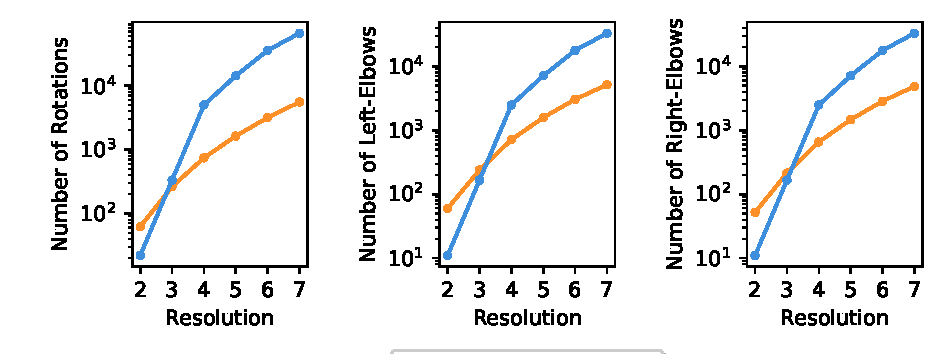
\includegraphics[width=16cm]{figures/phi4_hamiltonian_gates_vs_terms.pdf}
%     \caption{
%         \textbf{Numerical Gate Counts for Increasing $L$ ($\phi^4$ Hamiltonian).}
%         The number of rotations (left), left-elbows (middle), and right-elbows (right) are plotted as a function of the number of terms in the Hamiltonian ($L$) for an increasing number of momentum modes ($I$).
%         The gate counts for the variant of LOBE using \textit{USP} are shown as the blue squares.
%         The gate counts for the variant of LOBE using \textit{ASP} are shown as the orange circles.
%         The bosonic occupancy cutoff ($\Omega$) is set to $3$.
%         The number of rotations excludes rotations by angles that result in Clifford operations.
%     }
%     \label{fig:phi4_hamiltonian_gates_vs_terms}
% \end{figure}
% \begin{figure}
%     \centering
%     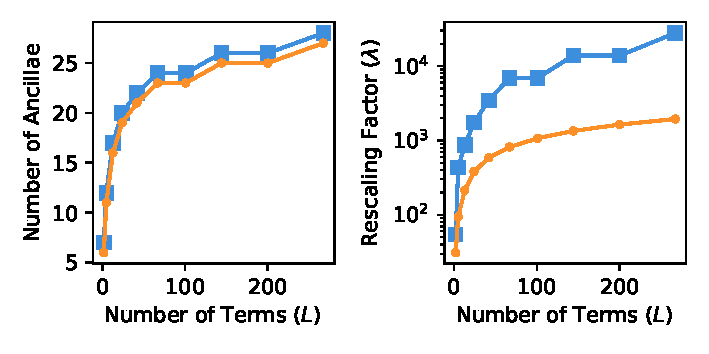
\includegraphics[width=12cm]{figures/phi4_hamiltonian_qubits_and_rescaling_vs_terms.pdf}
%     \caption{
%         \textbf{Numerical Ancillae Counts and Rescaling Factors for Increasing $L$ ($\phi^4$ Hamiltonian).}
%         The number of required ancillae (left) and the resulting rescaling factor (right) for LOBE are plotted as a function of the number of terms in the Hamiltonian ($L$) for an increasing number of momentum modes ($I$).
%         The counts for the variant of LOBE using \textit{USP} are shown as the blue squares.
%         The counts for the variant of LOBE using \textit{ASP} are shown as the orange circles.
%         The bosonic occupancy cutoff ($\Omega$) is set to $3$.
%     }
%     \label{fig:phi4_hamiltonian_qubits_and_rescaling_vs_terms}
% \end{figure}

% \begin{figure}
%     \centering
%     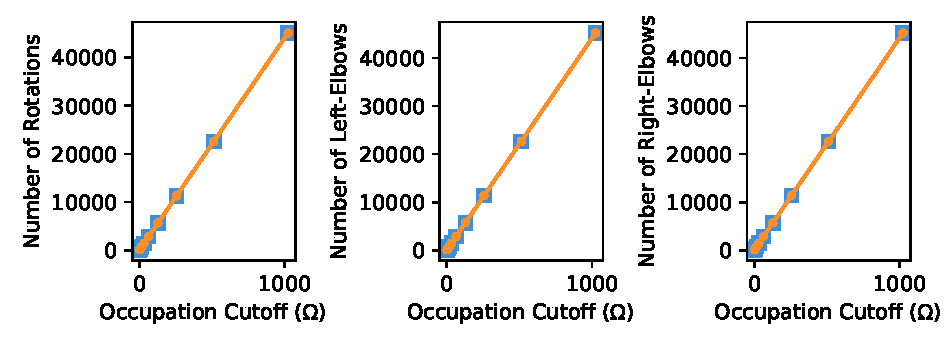
\includegraphics[width=16cm]{figures/phi4_hamiltonian_gates_vs_omega.pdf}
%     \caption{
%         \textbf{Numerical Gate Counts for Increasing $\Omega$ ($\phi^4$ Hamiltonian) .}
%         The number of rotations (left), left-elbows (middle), and right-elbows (right) are plotted as a function of the bosonic occupation cutoff ($\Omega$).
%         The gate counts for the variant of LOBE using \textit{USP} are shown as the blue squares.
%         The gate counts for the variant of LOBE using \textit{ASP} are shown as the orange circles.
%         The number of momentum modes ($I$) is set to $3$.
%         The number of rotations excludes rotations by angles that result in Clifford operations.
%     }
%     \label{fig:phi4_hamiltonian_gates_vs_omega}
% \end{figure}
% \begin{figure}
%     \centering
%     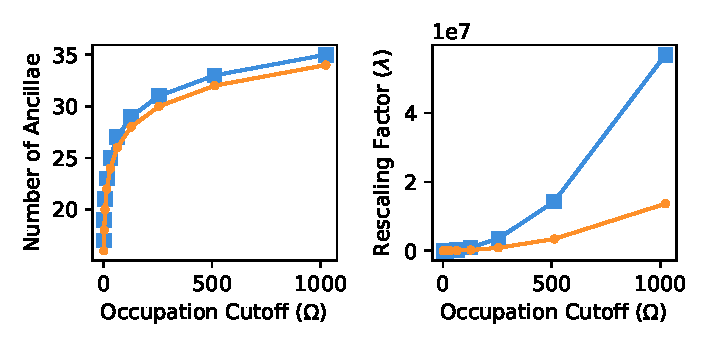
\includegraphics[width=12cm]{figures/phi4_hamiltonian_qubits_and_rescaling_vs_omega.pdf}
%     \caption{
%         \textbf{Numerical Ancillae Counts and Rescaling Factors for Increasing $\Omega$ ($\phi^4$ Hamiltonian).}
%         The number of required ancillae (left) and the resulting rescaling factor (right) for LOBE are plotted as a function of the bosonic occupation cutoff ($\Omega$).
%         The counts for the variant of LOBE using \textit{USP} are shown as the blue squares.
%         The counts for the variant of LOBE using \textit{ASP} are shown as the orange circles.
%         The number of momentum modes ($I$) is set to $3$.
%     }
%     \label{fig:phi4_hamiltonian_qubits_and_rescaling_vs_omega}
% \end{figure}